\documentclass[11pt]{article}
\usepackage[margin=0.7in]{geometry}
\usepackage{amsmath,amssymb}
\usepackage{enumitem}
\usepackage{tikz}
\usepackage{pgfplots}
\pgfplotsset{compat=1.18}
\usepackage{fancyhdr}
\usepackage{parskip}
\setlist[enumerate]{leftmargin=*, itemsep=6pt}
\pagestyle{fancy}
\fancyhf{}
\fancyfoot[L]{\small\textit{en}Vision\textsuperscript{\textregistered} Algebra 2}
\fancyfoot[C]{\small 4-2 Lesson Quiz, short form}
\fancyfoot[R]{\small\thepage}
\renewcommand{\headrulewidth}{0pt}
\newcommand{\choice}[1]{\tikz[baseline=-0.6ex]\node[draw, circle, inner sep=0.6pt, minimum size=3.3mm, font=\scriptsize\bfseries] {#1};\;}
\newcommand{\checkbox}{$\square$\;}
\pgfplotsset{quizgrid/.style={
  axis lines=middle, grid=both, grid style={gray!45},
  ticklabel style={font=\scriptsize, fill=white, inner sep=1pt},
  xlabel={$x$}, ylabel={$y$}, axis line style={thick}, clip=true}}

\begin{document}

\noindent\textbf{Name}\; \rule{6cm}{0.4pt} \hfill Period \rule{1.2cm}{0.4pt} \quad Date \rule{2.2cm}{0.4pt}

\vspace{4pt}\noindent\rule{\textwidth}{0.6pt}

\vspace{2pt}\noindent{\LARGE\textbf{4-2 \; Lesson Quiz: Graphing Rational Functions}} \hfill {\small short form}

\vspace{4pt}\noindent\rule{\textwidth}{0.6pt}

{\small Question numbers match the Savvas Lesson Quiz. Questions 2 and 4 are not on this form.}

\vspace{4pt}
\begin{minipage}[t]{0.56\textwidth}
\textbf{1.} Which equation is shown in the graph?

\vspace{4pt}
\begin{itemize}[leftmargin=1.2em, itemsep=6pt]
\item[] \choice{A} $p(x)=2-\dfrac{1}{2x-4}$
\item[] \choice{B} $p(x)=2+\dfrac{1}{2x+4}$
\item[] \choice{C} $p(x)=2-\dfrac{1}{2x+4}$
\item[] \choice{D} $p(x)=2+\dfrac{1}{2x-4}$
\end{itemize}

\vspace{4pt}
The asymptotes I see on the graph: \;$x=\rule{1cm}{0.4pt}$ \quad $y=\rule{1cm}{0.4pt}$
\end{minipage}\hfill
\begin{minipage}[t]{0.42\textwidth}
\vspace{-6pt}
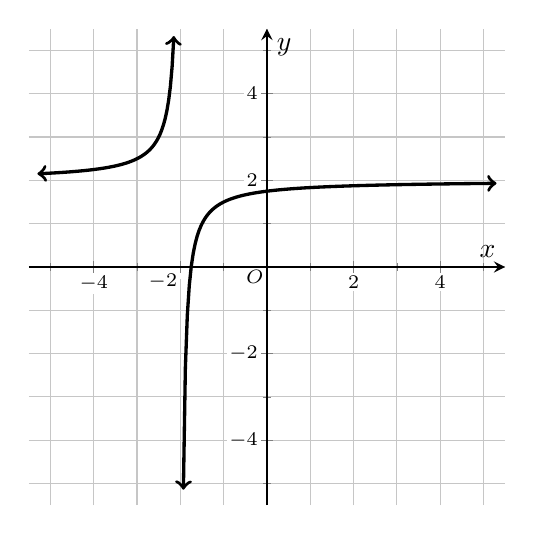
\begin{tikzpicture}
% TE window -5 to 5 plus half a unit of padding; labels -4,-2,2,4; unit grid; O at the origin.
% The -2 x-label is drawn by hand left of the grid line x = -2, because the right branch crosses
% the x-axis just right of it (at x = -1.75).
\begin{axis}[quizgrid, xmin=-5.5, xmax=5.5, ymin=-5.5, ymax=5.5,
  xtick={-4,-2,2,4}, xticklabels={$-4$,,$2$,$4$}, ytick={-4,-2,2,4},
  minor xtick={-5,...,5}, minor ytick={-5,...,5}, x=0.55cm, y=0.55cm]
\node[font=\scriptsize, fill=white, inner sep=1pt, anchor=north east] at (axis cs:-2,-0.08) {$-2$};
\node[font=\scriptsize, fill=white, inner sep=1pt, anchor=north east] at (axis cs:0,0) {$O$};
\addplot[very thick, <->, domain=-5.3:-2.15, samples=80] {2-1/(2*x+4)};
\addplot[very thick, <->, domain=-1.93:5.3, samples=160] {2-1/(2*x+4)};
\end{axis}
\end{tikzpicture}
\end{minipage}

\vspace{8pt}\noindent\rule{\textwidth}{0.4pt}

\vspace{6pt}
\textbf{3.} What are the vertical and horizontal asymptotes of the graph of $f(x)=\dfrac{3-2x}{4-3x}$?

\vspace{4pt}
\begin{minipage}[t]{0.40\textwidth}
\begin{itemize}[leftmargin=1.2em, itemsep=8pt]
\item[] \choice{A} $x=\frac43$ and $y=\frac23$
\item[] \choice{B} $x=\frac23$ and $y=\frac43$
\item[] \choice{C} $x=\frac34$ and $y=\frac23$
\item[] \choice{D} $x=\frac32$ and $y=\frac43$
\end{itemize}
\end{minipage}\hfill
\begin{minipage}[t]{0.56\textwidth}
\raggedright
Show your work.

\vspace{4pt}
Vertical asymptote (where is the denominator 0?):

\vspace{14pt}\rule{\linewidth}{0.4pt}

\vspace{8pt}
Horizontal asymptote (compare degrees, then leading coefficients):

\vspace{14pt}\rule{\linewidth}{0.4pt}
\end{minipage}

\vspace{10pt}\noindent\rule{\textwidth}{0.4pt}

\vspace{6pt}
\textbf{5.} The graph of which equation below has a horizontal asymptote at $y=-3$?

\vspace{4pt}
\begin{minipage}[t]{0.40\textwidth}
\begin{itemize}[leftmargin=1.2em, itemsep=8pt]
\item[] \choice{A} $y=\dfrac{x-3}{x+1}$
\item[] \choice{B} $y=\dfrac{x}{2-3x}$
\item[] \choice{C} $y=\dfrac{1-3x}{2+x}$
\item[] \choice{D} $y=\dfrac{1+3x}{2-3x}$
\end{itemize}
\end{minipage}\hfill
\begin{minipage}[t]{0.56\textwidth}
Write the horizontal asymptote of each choice.

\vspace{8pt}
A: $y=\rule{1.2cm}{0.4pt}$ \qquad B: $y=\rule{1.2cm}{0.4pt}$

\vspace{12pt}
C: $y=\rule{1.2cm}{0.4pt}$ \qquad D: $y=\rule{1.2cm}{0.4pt}$

\vspace{12pt}
Explain in one sentence how you found them.

\vspace{14pt}\rule{\linewidth}{0.4pt}
\end{minipage}

\vfill
\noindent\textbf{Scoring:} Question 3 and Question 5 are 10 points each. Question 1 is a bonus of up to 5 points. Total out of 20.

\newpage
\noindent{\LARGE\textbf{4-2 Lesson Quiz, short form: answer key}}

\vspace{4pt}\noindent\rule{\textwidth}{0.6pt}

\begin{enumerate}
\item[\textbf{1.}] \textbf{C, $p(x)=2-\dfrac{1}{2x+4}$.} The graph has vertical asymptote $x=-2$ and horizontal asymptote $y=2$, so the denominator is $2x+4$ (rules out A and D). The right branch is \emph{below} $y=2$: at $x=0$, C gives $2-\frac14=1.75$ and B gives $2.25$. Savvas quiz item 1, DOK 1, Realize skill F20. Taught by Example 4 (asymptotes, then a test point). \textbf{Bonus 5:} 2 for both asymptotes written correctly, 3 for C.
\item[\textbf{3.}] \textbf{A, $x=\frac43$ and $y=\frac23$.} $4-3x=0$ gives $x=\frac43$ (the numerator is $3-2\cdot\frac43=\frac13\neq0$). Same degree, so $y=\frac{-2}{-3}=\frac23$. Savvas quiz item 3, DOK 1, Realize skill F76. Taught by Example 4. \textbf{10 points:} 6 for A, 2 for the vertical-asymptote work, 2 for the horizontal-asymptote work. Distractor B swaps the two; C solves $4x-3=0$; D uses the numerator.
\item[\textbf{5.}] \textbf{C, $y=\dfrac{1-3x}{2+x}$.} Every choice has equal degrees, so the asymptote is the ratio of leading coefficients: A $\frac11=1$; B $\frac{1}{-3}=-\frac13$; C $\frac{-3}{1}=-3$; D $\frac{3}{-3}=-1$. Savvas quiz item 5, DOK 2, Realize skill F76. Taught by Example 3 (Case 3). \textbf{10 points:} 6 for C, 3 for the four asymptotes (any three correct), 1 for the sentence naming degree and leading coefficients.
\end{enumerate}

\textbf{Items left off this form} (available for a retake or Form B):
Savvas item 2, vertical asymptotes of $y=\frac{(x+1)^2}{x^2-3x-4}$ (answer D, $x=4$ only: $x^2-3x-4=(x-4)(x+1)$ and $x+1$ is also a factor of the numerator, so $x=-1$ is not an asymptote; DOK 2, F76; taught by Examples 2 and 6, both cut);
Savvas item 4, water added to 10 liters of a 12\% salt mixture, $f(x)=\frac{1.2}{x+10}$, liters of water for a 1\% mixture (answer 110 liters: $\frac{1.2}{x+10}=0.01$ gives $x+10=120$; DOK 2, F74; taught by Example 5, cut; the packet's Practice block is its parallel). The TE prints item 4's function as a ``percent'' but it gives a fraction (0.01 for 1\%).

\textbf{IXL replacement:} SmartScore 70 or above on 7JJ and 79Q replaces this quiz with 20/20.

\end{document}
